\section{Result}
This section will look at the results in the form of calculated equations of motion and steady state solutions. Both with and without feedback. The first subsection will deal with a QHO which is measured continuously and without feedback, while the second subsection will add feedback into the scheme.
\subsection{Measurement Without Feedback}
Consider a QHO described by the Hamiltonian in Eq. \eqref{eq:hamiltonian} which is coupled to a thermal bath with temperature $T$. If the oscillator's position quadrature is also continuously measured the evolution of the system can be described by the master equation in Eq. \eqref{eq:masterMeas} using the Lindblad operators mentioned in Sec. \ref{sec:mastereq}. We want to solve for \gls{eom} when measuring for the position quadrature
\begin{align}
    \dt\expval{\xop^2} &= \tr(\xop^2 \dt \dmatrix)\label{eq:x2}, \\
    \dt\expval{\pop^2} &= \tr(\pop^2 \dt \dmatrix)\label{eq:p2},\\
    \dt\expval{\acomm{\xop}{\pop}} &= \tr(\acomm{\xop}{\pop} \dt \dmatrix). \label{eq:xp}
\end{align}
The choice of looking at the second momenta has to do with their relation to the variance and thus the fluctuations of the system. These fluctuations are then related to the energy contained in the oscillator. When looking at feedback control and interesting application is to minimize the energy in the oscillator and, which is thus also an argument for looking at the second momenta.
Solving Eqs. \eqref{eq:x2} to \eqref{eq:xp} yields the following EOM
\begin{align}
    \dt\expval{\xop^2} &= - \gamma \expval{\xop^2} - \frac{1}{m}\expval{\acomm{\xop}{\pop}} + \frac{\gamma \hbar}{m\omega}(\nbar + 1/2),\\
    \dt\expval{\pop^2} &= -\gamma \expval{\pop^2} + m\omega^2 \expval{\acomm{\xop}{\pop}} + \gamma m \omega\hbar (\nbar + 1/2) + \lambda \hbar^2,\\
    \dt\expval{\acomm{\xop}{\pop}} &= -\gamma \expval{\acomm{\xop}{\pop}} + 2 m \omega^2 \expval{\xop^2} - \frac{2}{m} \expval{\pop^2}
\end{align}
for more detailed calculations see App. \ref{app:eom}. Performing a change of variable to make the equations dimensionless
\begin{equation}
    \tilde{x} = \sqrt{\frac{m\omega}{\hbar}} x \quad \text{and} \quad \tilde{p} = \sqrt{\frac{1}{m \omega \hbar}} p ,
\end{equation}
we can solve for the steady state. By introducing the quality factor $Q = \omega / \gamma$ we obtain the steady state solutions
\begin{align}
    \expval{\tilde{x}^2}_\mathrm{ss} &= (\nbar + 1/2) + \frac{\lambda \hbar}{m \omega^2} \frac{2 Q^3}{4Q^2 + 1}, \label{eq:x2ss}\\
    \expval{\tilde{p}^2}_\mathrm{ss} &= (\nbar + 1/2) + \frac{\lambda \hbar}{m \omega^2} \left( Q - \frac{2Q^3}{4Q^2 + 1} \right) \label{eq:p2ss},\\
\end{align}
One interesting aspects of the equations is that both equations have identical terms capturing the thermal aspect of the fluctuations. Another interesting thing is that without measurement the equations are only thermal, which is to be expected. Interestingly, when calculating the energy of the steady state the complicated fraction disappears and we are left with a purely linear term in the quality factor.
\begin{equation}
    E_\mathrm{ss} = \expval{\tilde{H}}_\mathrm{ss} = \frac{\hbar \omega}{2} \left( \expval{\tilde{p}^2} + \expval{\tilde{x}^2} \right) = \hbar\omega (\nbar + 1/2)+ \frac{\lambda \hbar^2}{2 m\omega} Q
    \label{eq:ess}
\end{equation}

\begin{figure}
    \centering
    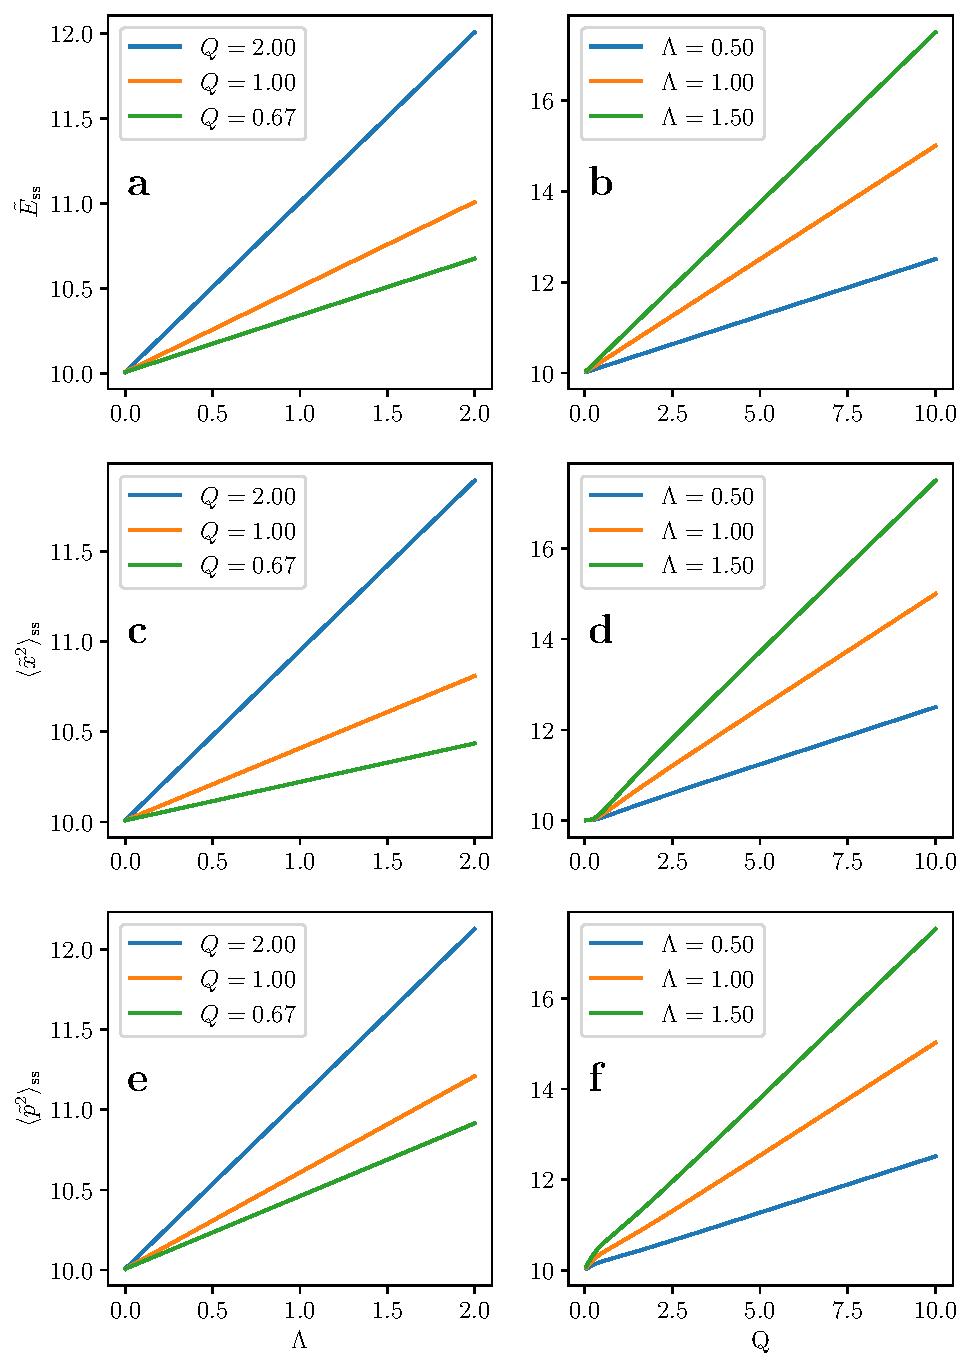
\includegraphics[width=\textwidth]{measurement_result.pdf}
    \caption{ \small The top panels show Eq. \eqref{eq:ess}, the middle panels show Eq. \eqref{eq:x2ss} and the bottom panels show Eq. \eqref{eq:p2ss}. All plots use the parameters $k_\mathrm{B}T = 10$ and $\omega = \hbar = 1$. The left panels are plotted against $\lambda / \omega$ and with three different values for $Q$, while the right panels are plotted against $Q$ and three different values of $\lambda$. }
    \label{fig:steady_state}
\end{figure}

Looking at panels \textbf{a} and \textbf{b} in Fig. \ref{fig:steady_state} one can see that a stronger measurement correlates to the system steady state increasing in energy, as does it for an increasing quality factor. Both also affect the system linearly. Thus, by continuously measuring the system we add energy into it, which make the steady state higher in energy than what the thermal effects from the bath would otherwise place it. That is, if we do not perform any measurement the system would be stable at around $\nbar + 1/2$ which for the parameters used here would give $\expval{\tilde{E}} \approx 10\hbar\omega$

In panels \textbf{d} and \textbf{f} we can see that there is some non-linear behaviour near $Q = 0$. However, due to the approximations made in Sec. \ref{sec:open} we cannot trust the results in the region of a low quality factor. Due to this regime having a relatively high coupling to the environment, and thus the excitations in the environment might not decay fast enough and therefore affect the oscillator. Panels \textbf{c} and \textbf{e} show the linear dependence on $\lambda$ for the second momenta.

Using the same master equation as above we can also solve for the first momenta
\begin{align}
    \dt\expval{\xop} &= \tr(\xop \dt \dmatrix),\\
    \dt\expval{\pop} &= \tr(\pop \dt \dmatrix).
\end{align}
Solving these equations we find 
\begin{align}
    \dt\expval{\xop} &= -\frac{\gamma}{2} \expval{\xop} - \frac{1}{m} \expval{\pop},\\
    \dt\expval{\pop} &= -\frac{\gamma}{2} \expval{\pop} + m\omega^2 \expval{x}.
\end{align}
Then when solving for the steady state we find 
\begin{equation}
    \expval{\xop} = \expval{\pop} = 0. \label{eq:xp0}
\end{equation}
This result also confirms the intuition that for a harmonic oscillator, the system has a steady state around the origin. To check for stability we can rewrite the equation as an eigenvalue problem and solve for the eigenvalues. That is, for the matrix
\begin{equation}
    \mathcal{M} = \begin{pmatrix}
        -\gamma/2 & -1/m \\
        m\omega^2 & -\gamma/2
    \end{pmatrix}
\end{equation}
the eigenvalues are 
\begin{align}
    \lambda_1 &= -\frac{\gamma}{2} - i\omega,\\
    \lambda_2 &= -\frac{\gamma}{2} + i\omega.
\end{align}
Since the real part of the eigenvalues are negative the system is stable.

Eq. \eqref{eq:xp0} also shows that the variance of the system is only dependent on the first momenta, since
\begin{equation}
    \sigma^2_{\hat{A}} = \expval{\hat{A}^2} - \expval{\hat{A}}^2
\end{equation}
for an operator $\hat{A}$. It is also an easy calculation then to show that for temperature $T=0$ and without measurement we have equality in the Heisenberg uncertainty relation, justifying the accuracy of the results, and the approximations made in the derivation of the master equation.

\subsection{Feedback}
We now consider a feedback mechanism on the oscillator described by Eq. \eqref{eq:masterFeed} which is a linear feedback scheme. Solving for the first momenta's EOM we find 
\begin{align}
    \dt\expval{\xop} &= - \left(\frac{\gamma}{2} + \frac{2 \im{f}}{\sqrt{2 m \omega \hbar}} \right)\expval{\xop} - \frac{1}{m} \expval{\pop},\\
    \dt\expval{\pop} &= -\frac{\gamma}{2}\expval{\pop} + \left(\re{f} \sqrt{\frac{2 m \omega}{\hbar}} + m \omega^2 \right) \expval{\xop}.
\end{align}
Choosing $f$ such that
\begin{equation}
    \re{f} = - \sqrt{\frac{m \omega^3 \hbar}{2}} \quad \text{and} \quad \im{f} = -\frac{\gamma\sqrt{m\omega\hbar}}{2\sqrt{2}} \label{eq:reFimF_toZero}
\end{equation}
The system of equations reduces to
\begin{align}
    \dt\expval{\xop} &= - \frac{1}{m} \expval{\pop},\\
    \dt\expval{\pop} &= -\frac{\gamma}{2} \expval{\pop},
\end{align}
which has a steady state solution for $\expval{\pop} = 0$ and any $\expval{\xop}$. To check for stability we can again rewrite the equations as an eigenvalue problem with matrix
\begin{equation}
    \mathcal{M} = 
    \begin{pmatrix}
        - \left(\frac{\gamma}{2} + \frac{2 \im{f}}{\sqrt{2 m \omega \hbar}} \right) & - \frac{1}{m} \\
        -\frac{\gamma}{2} & \re{f} \sqrt{\frac{2 m \omega}{\hbar}} + m \omega^2
    \end{pmatrix},
\end{equation}
which has eigenvalues
\begin{equation}
    \lambda_\pm = \frac{\pm \sqrt{2} \sqrt{ -m^2 \left( 2 \sqrt{2} \re{f} \omega \hbar \sqrt{\frac{m\omega}{\hbar}} + 2 m \omega^3 \hbar - \im{f}^2 \right) } -\sqrt{2} m \im{f} - \gamma m \sqrt{m \omega \hbar} }{ 2 m \sqrt{ m \omega \hbar}}.
\end{equation}
Inserting the values of $\re{f}$ and $\im{f}$ from Eq. \eqref{eq:reFimF_toZero} we find the eigenvalues to be $\lambda_\pm = \pm \gamma$, showing us that the system is not always stable. We could interpret this result as the potential following the particle and having its minimum at $\expval{\xop}$ so the particle can move as a free particle.

Solving for the EOM for the second momenta we obtain
\begin{align}
    \dt \expval{x^2} &= -\left(\gamma + \frac{4\im{f}}{\sqrt{2 m \omega \hbar}}\right) \expval{x^2} - \frac{1}{m} \expval{\acomm{x}{p}} + \frac{\gamma \hbar}{m \omega} (\nbar + 1/2) - \frac{1}{4\lambda m \omega \hbar} \re{f}^2,\\
    \dt \expval{p^2} &=  -\gamma \expval{p^2} + \left( m\omega^2 - \re{f} \sqrt{\frac{2m \omega}{\hbar}} \right)\expval{\acomm{x}{p}} + \gamma m \omega \hbar (\nbar + 1/2) + \lambda \hbar^2 + \frac{m \omega}{4 \lambda \hbar}\re{f}^2 ,\\
    \dt \expval{\acomm{x}{p}} &= \left(\frac{2}{\sqrt{2m \omega \hbar}}\im{f} - \gamma  \right)\expval{\acomm{x}{p}} + \left(2 m \omega^2 + 2 \sqrt{\frac{2 m \omega}{\hbar}}\re{f} \right) \expval{x^2} - \frac{2}{m} \expval{p^2} - \frac{\re{f} \im{f}}{2 \lambda \hbar}.
\end{align}
Performing the same change of variables as earlier with addition of 
\begin{equation}
    \re{\tilde{f}} = \sqrt{\frac{2 m}{\hbar \omega}} \re{f} \quad \text{and} \quad \im{\tilde{f}} = \frac{1}{\sqrt{2 m \omega \hbar}} \im{f}, 
\end{equation}
we can solve for the steady state. First we define
\begin{equation}
    D = 8m\lambda ( -\gamma ( -2\im{\tilde{f}} + \gamma ) (4\im{\tilde{f}} + \gamma)+ 8\im{\tilde{f}}\im{\tilde{f}} \omega - 4 (2\im{\tilde{f}} + \gamma)\omega^2 )\hbar
\end{equation}
then we can write the solutions as
\begin{multline}
    \expval{\tilde{x}^2} = \frac{1}{D} (\re{\tilde{f}} \omega (-2 \im{\tilde{f}} \gamma ( \re{\tilde{f}} - 2m \omega ) + \re{\tilde{f}} (\gamma^2 - 2 \re{\tilde{f}} \omega) ) \\ -8m (\nbar + 1/2)\gamma \lambda(-2\im{\tilde{f}}\gamma + \gamma^2 - 2(\re{\tilde{f}}- 2\omega)\omega )\hbar
\end{multline}
\begin{multline}
    \expval{\tilde{p}^2} = \frac{1}{D} (\re{\tilde{f}} \omega ( -2 \re{\tilde{f}}^3 + \re{\tilde{f}} ( \im{\tilde{f}}(2 + 4m) - \gamma )(4 \im{\tilde{f}} + \gamma) \\- 2( \re{\tilde{f}}^2 + 2 \im{\tilde{f}} m (4 \im{\tilde{f}} + \gamma) ) \omega ) \\- 8m(\nbar + 1/2) \gamma \lambda ( -8 \im{\tilde{f}}^2 + 2 \im{\tilde{f}} \gamma + \gamma^2 - 2 (\re{\tilde{f}} - 2 \omega)(\re{\tilde{f}} + \omega) ) \hbar
    ) 
\end{multline}
\begin{multline}
    \expval{\acomm{\tilde{x}}{\tilde{p}}} = \frac{1}{2D} (\re{\tilde{f}} \omega ( -8 \im{\tilde{f}}^2 m \gamma + \re{\tilde{f}} \gamma (\re{\tilde{f}} + 2 \omega) \\+ \im{\tilde{f}} (-2 m \gamma^2 + 4 \re{\tilde{f}} \omega) ) - 8 m (\nbar + 1/2) \gamma \lambda (\re{\tilde{f}} \gamma - 4 \im{\tilde{f}} \omega) \hbar
    )
\end{multline}